\documentclass{article}

\usepackage[margin=1in]{geometry}
\usepackage{amsmath}
\usepackage{graphicx}

\author{Damien Prieur}
\title{Assignment 1 \\ CS 435}
\date{}

\catcode`\%=12
\newcommand\pcnt{%}
\catcode`\%=14

\begin{document}

\maketitle

\section*{Question 1}
\begin{enumerate}
\item (2pts) Given a point in 3D space, (3,5,20) and an effective focal length of 10, where will this point appear on the 2D image plane?
\\
We can solve this using the lens formula solving for x and y independently.
$$ \frac{y'}{y} = \frac{z'}{z} $$
$$ z' = 10 \qquad z = 20 \qquad \Rightarrow \qquad e_1'(e_1) = e_1 \frac{10}{20} $$
So we get this function
$$ (x,y,z) \Rightarrow (e_1'(x), e_1'(y), e_1'(z)) $$
Plugging in our numbers we get
$$ (3,5,20) \Rightarrow (1.5,2.5,10) $$

So it will appear at $ x = 1.5 $ and $ y = 2.5 $ on our 2D image plane.


\item (2pts) If we have a focal length of 10 and a lens effective diameter of 5, what is the field of view of this camera system (in degrees)?
\\
We can solve this using the Field of View formula.
$$ \tan\left(\frac{\theta}{2}\right)=\frac{D}{2f} $$
Based on the problem we have $D = 5 $ and $ f = 10 $
Solving for $\theta$ we get
$$ \theta = 2\arctan\left(\frac{D}{2f}\right) $$
Plugging in we get

$$ \theta = 2\arctan\left(\frac{5}{2\times10}\right) \approx 28.1\text{ degrees}$$

\item   Based on observing a histogram perhaps we decided to create the following pixel intensity mappings in order to stretch the values of a particularly compressed area (you may assume the full range is [0,255]):\\

\begin{center}
[0,20]$\rightarrow$[0,10]\\
(20,25]$\rightarrow$(10,95]\\
(25,100)$\rightarrow$(95,100]
\end{center}

\begin{enumerate}
\item(2pts) Draw a 2D graph showing these mappings.  The x-axis will be the input values and the y-axis will be the output values.
\begin{figure}[h]
    \centering
    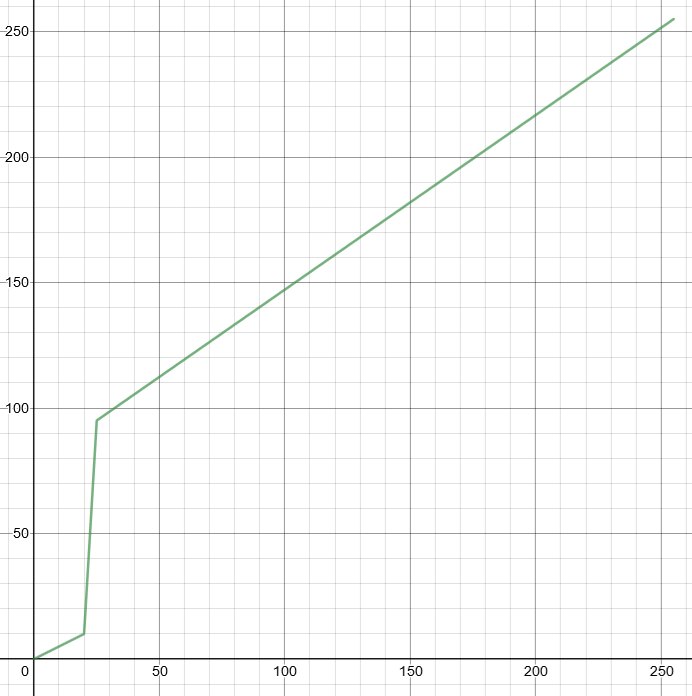
\includegraphics[scale=.5]{images/1-3-a.png}
\end{figure}


\item (3pts) What are the equations for these mappings?
$$ f(x) = \begin{cases}
    \frac{10-0}{20-0} (x-0) + 0 & 0 \leq x \leq 20 \\
    \frac{95-10}{25-20}(x-20) + 10 & 20 < x \leq 25 \\
    \frac{100-95}{100-25}(x-25) + 95 & 25 < x \leq 100 \\
    x & 100 < x \leq 255
 \end{cases} $$
Simplifying gives us
$$ f(x) = \begin{cases}
    \frac{x}{2} & 0 \leq x \leq 20 \\
    17x-330 & 20 < x \leq 25 \\
    \frac{x}{15}+\frac{280}{3} & 25 < x \leq 100 \\
    x & 100 < x \leq 255
 \end{cases} $$

\item (1pt) Given a value of 50, what will this value be mapped to?
$$f(50) = \frac{50}{15}+\frac{280}{3} = \frac{1450}{15} \approx 96.7 $$
\end{enumerate}
\end{enumerate}

\section*{Question 2}
The first point-processing thing we want to be able to do is to convert an image from color to grayscale.\\

\noindent
Read in your color image and use the following formula to convert it to a grayscale image.  You \textbf{may not} use a built-in function to do this (i.e rgb2gray).\\

\begin{equation}
Gray=0.2989R+0.5870*G+0.1140B
\end{equation}
\begin{figure}[h]
    \centering
    \includegraphics[scale=.5]{images/generated/Q2_grayscale.png}
\end{figure}


\section*{Question 3}
In this part, we want to be able to convert our color image (or grayscale image) into a binary image, where each pixel is either black or white.\\

\noindent
Produce three binary images, one for each of the following thresholds (as percentages of maximum possible intensity value):
\begin{itemize}
\item t=25\%
\begin{figure}[h!]
    \includegraphics[scale=.25]{images/generated/Q3_threshold25\pcnt.png}
\end{figure}
\item t=50\%
\begin{figure}[h]
    \includegraphics[scale=.5]{images/generated/Q3_threshold50\pcnt.png}
\end{figure}
\item t=75\%
\begin{figure}[h]
    \includegraphics[scale=.5]{images/generated/Q3_threshold75\pcnt.png}
\end{figure}
\end{itemize}


\section*{Question 4}
Histograms are a critical analysis tool use for many computer vision problems.  Display four histograms for your image, each of which have 256 bins.  \textbf{You may not use a built-in function to obtain the histogram}.  To plot your histogram, use the \emph{bar} function of Matlab.

\begin{itemize}
\item Grayscale histogram
\begin{figure}
    \includegraphics[width=\linewidth]{images/generated/Q4_hist_gray.png}
\end{figure}
\item Histogram of the red channel
\begin{figure}
    \includegraphics[width=\linewidth]{images/generated/Q4_hist_red.png}
\end{figure}
\item Histogram of the green channel
\begin{figure}
    \includegraphics[width=\linewidth]{images/generated/Q4_hist_green.png}
\end{figure}
\item Histogram of the blue channel.
\begin{figure}
    \includegraphics[width=\linewidth]{images/generated/Q4_hist_blue.png}
\end{figure}
\end{itemize}


\section*{Question 5}
Finally, we want to use the grayscale histogram in the previous part to perform contrast stretching.   Based on your histogram, perform contrast stretching.  It will be up to you to decide on the region mappings and how many there should be.  Again, this should be driven by your histograms in the previous part.\\

\noindent
Your submission should include:
\begin{itemize}
\item The original grayscale image and its histogram.
\begin{figure}
    \includegraphics[width=\linewidth]{images/generated/Q2_grayscale.png}
\end{figure}
\begin{figure}
    \includegraphics[width=\linewidth]{images/generated/Q4_hist_gray.png}
\end{figure}
\item The contrast stretched grayscale image and its histogram.
\begin{figure}
    \includegraphics[width=\linewidth]{images/generated/Q5_grayscale_contrast_stretched.png}
\end{figure}
\begin{figure}
    \includegraphics[width=\linewidth]{images/generated/Q5_hist_contrast_stretched.png}
\end{figure}
\item \textbf{A list of the region mappings along with text justifying your decision}.
\end{itemize}
Based on the initial histogram i decided to remove the regions that were not at all being used and stretch the rest of the regions outwards.
This lead me to have this mapping
$$ [26, 245] \Rightarrow [0,255] $$


\end{document}
